\documentclass[14pt, a4paper]{article}
\usepackage{mathtext}
\usepackage[T2A]{fontenc}
\usepackage[utf8]{inputenc}
\usepackage[russian]{babel}
\usepackage{multirow}
\usepackage{slashbox}
\usepackage{makecell}
\usepackage{graphicx}
\usepackage{physics}
\usepackage{amstext}
\usepackage{caption}
\usepackage{subcaption}
\usepackage{cmap}
\usepackage{float}
\usepackage{indentfirst}

\usepackage[a4paper,
            		left=1in,
            		right=1in,
           		 top=1in,
            		bottom=1in,
            		footskip=.25in]{geometry}

\renewcommand{\thesection}{\arabic{section}.}
\renewcommand{\thesubsection}{\arabic{section}.\arabic{subsection}.}

\title{\textbf{Отчет о выполнении лабораторной работы 17 "Демодуляция в шумах"}}
\author{Калашников Михаил, Б03-202}
\date{}

\begin{document}
\maketitle

\section{Канал с двоичной фазовой модуляцией}

\begin{figure}[H]
\centering
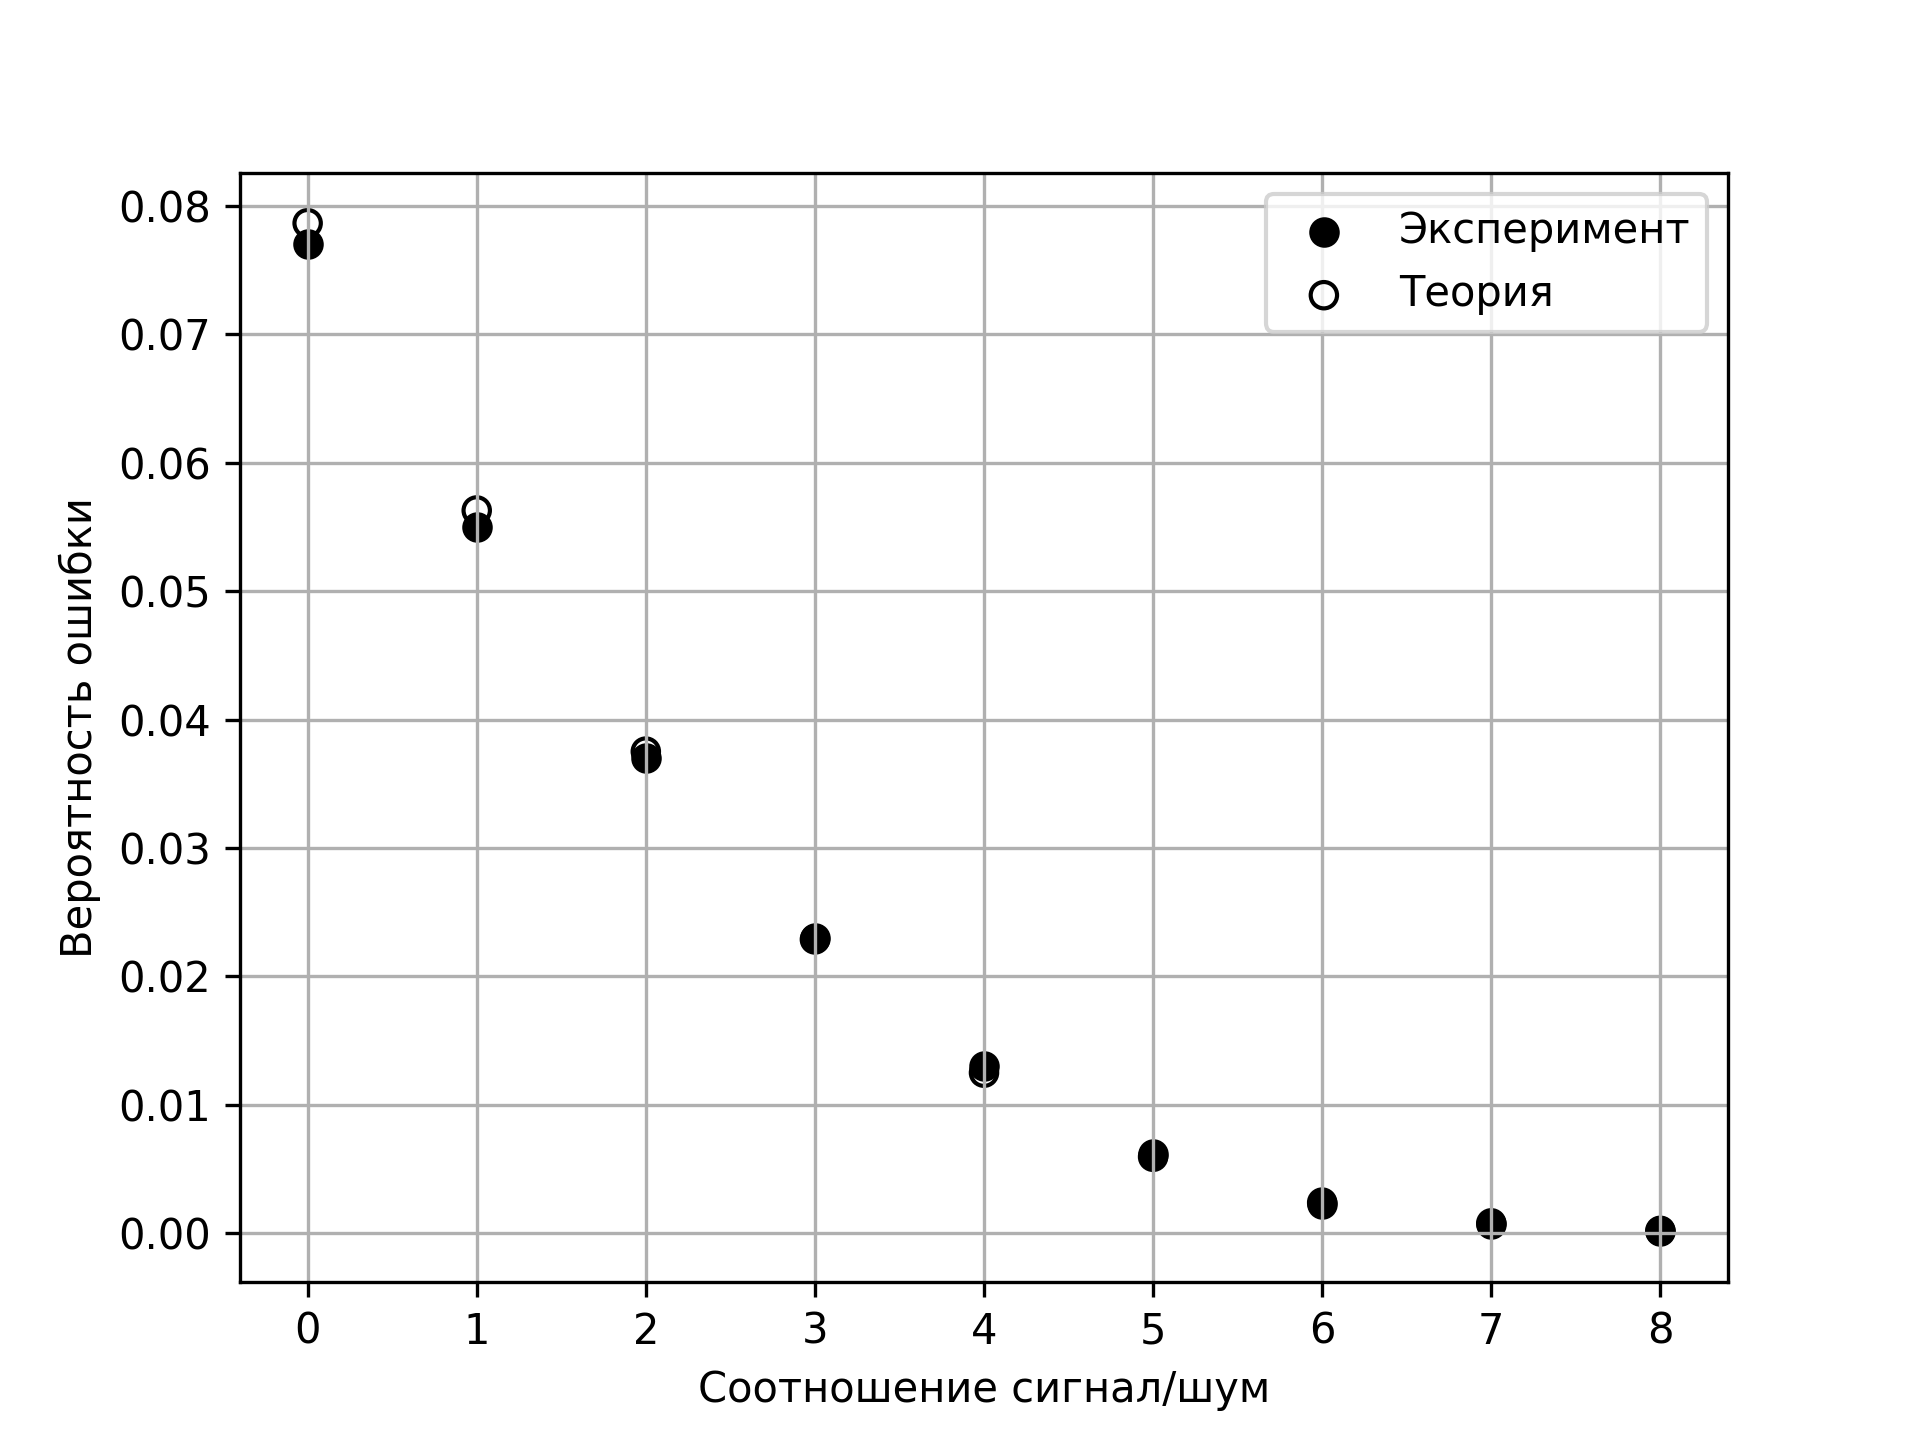
\includegraphics[width=.6\linewidth]{../images/rt2-1}
\end{figure}

Повернем созвездие на угол $\frac{\pi}{4}$. При $\text{snr}=6\ \text{dB}$, получим, что $P_e^\prime\approx0.023$. Как видно из графика, при $\text{snr}=3\ \text{dB}$ вероятность ошибки изначального созвездия так же составляет $P_e\approx0.023$.

\section{Канал с двоичной ортогональной модуляцией}

\begin{figure}[H]
\centering
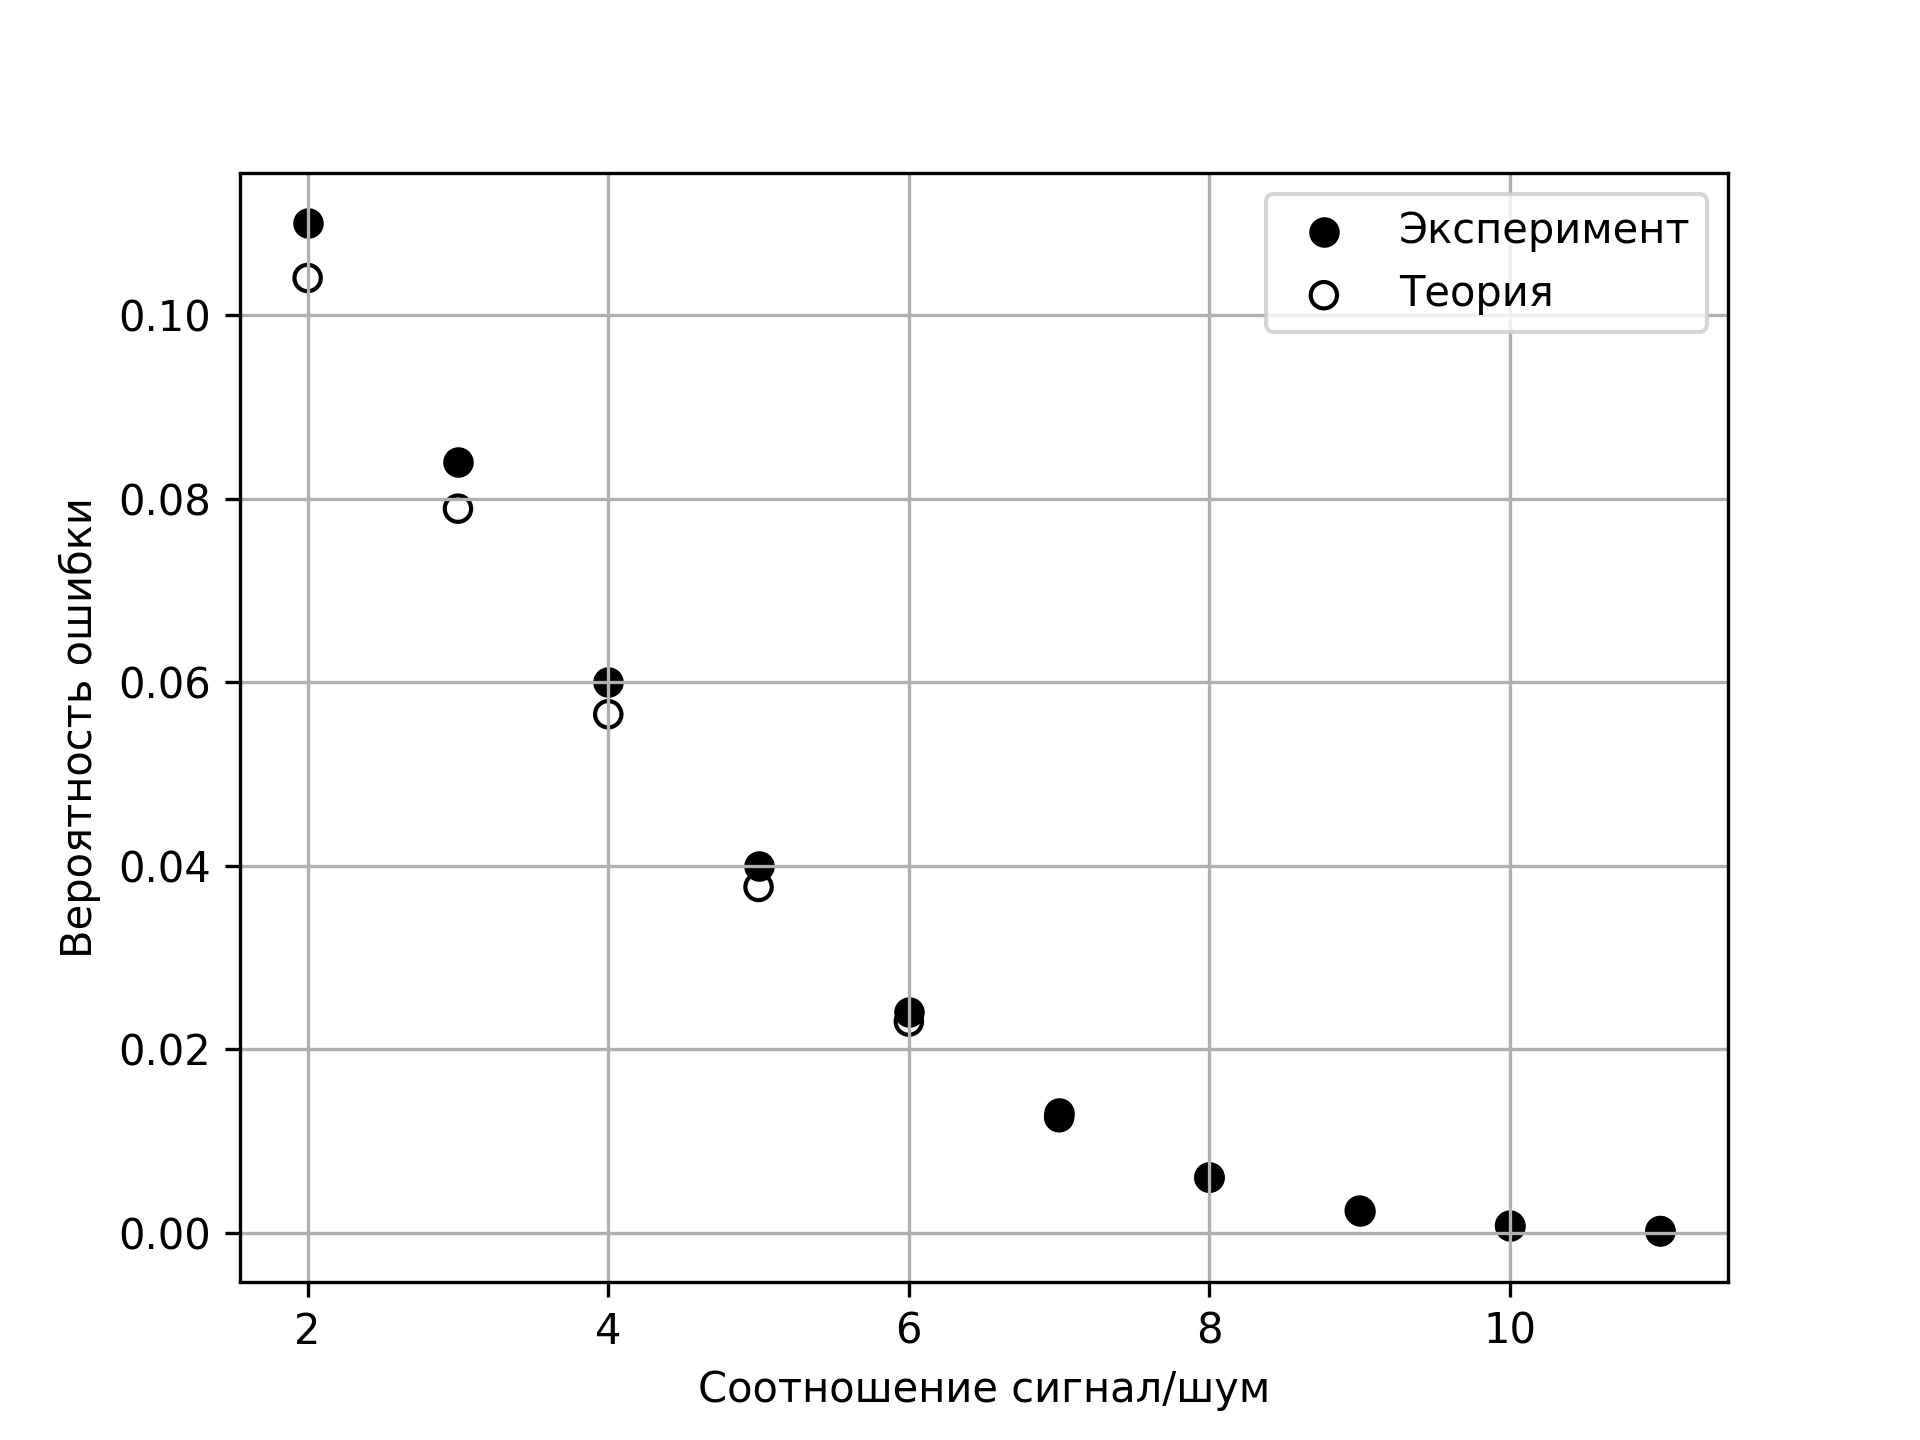
\includegraphics[width=.6\linewidth]{../images/rt2-2}
\end{figure}

Повернем созвездие на угол $\frac{\pi}{8}$. При $\text{snr}=6\ \text{dB}$, получим, что $P_e^\prime\approx0.071$. Это примерно соответствует значению $\text{snr}\approx3.5\ \text{dB}$.

\section{Канал с двоичной амплитудной модуляцией}

\begin{figure}[H]
\centering
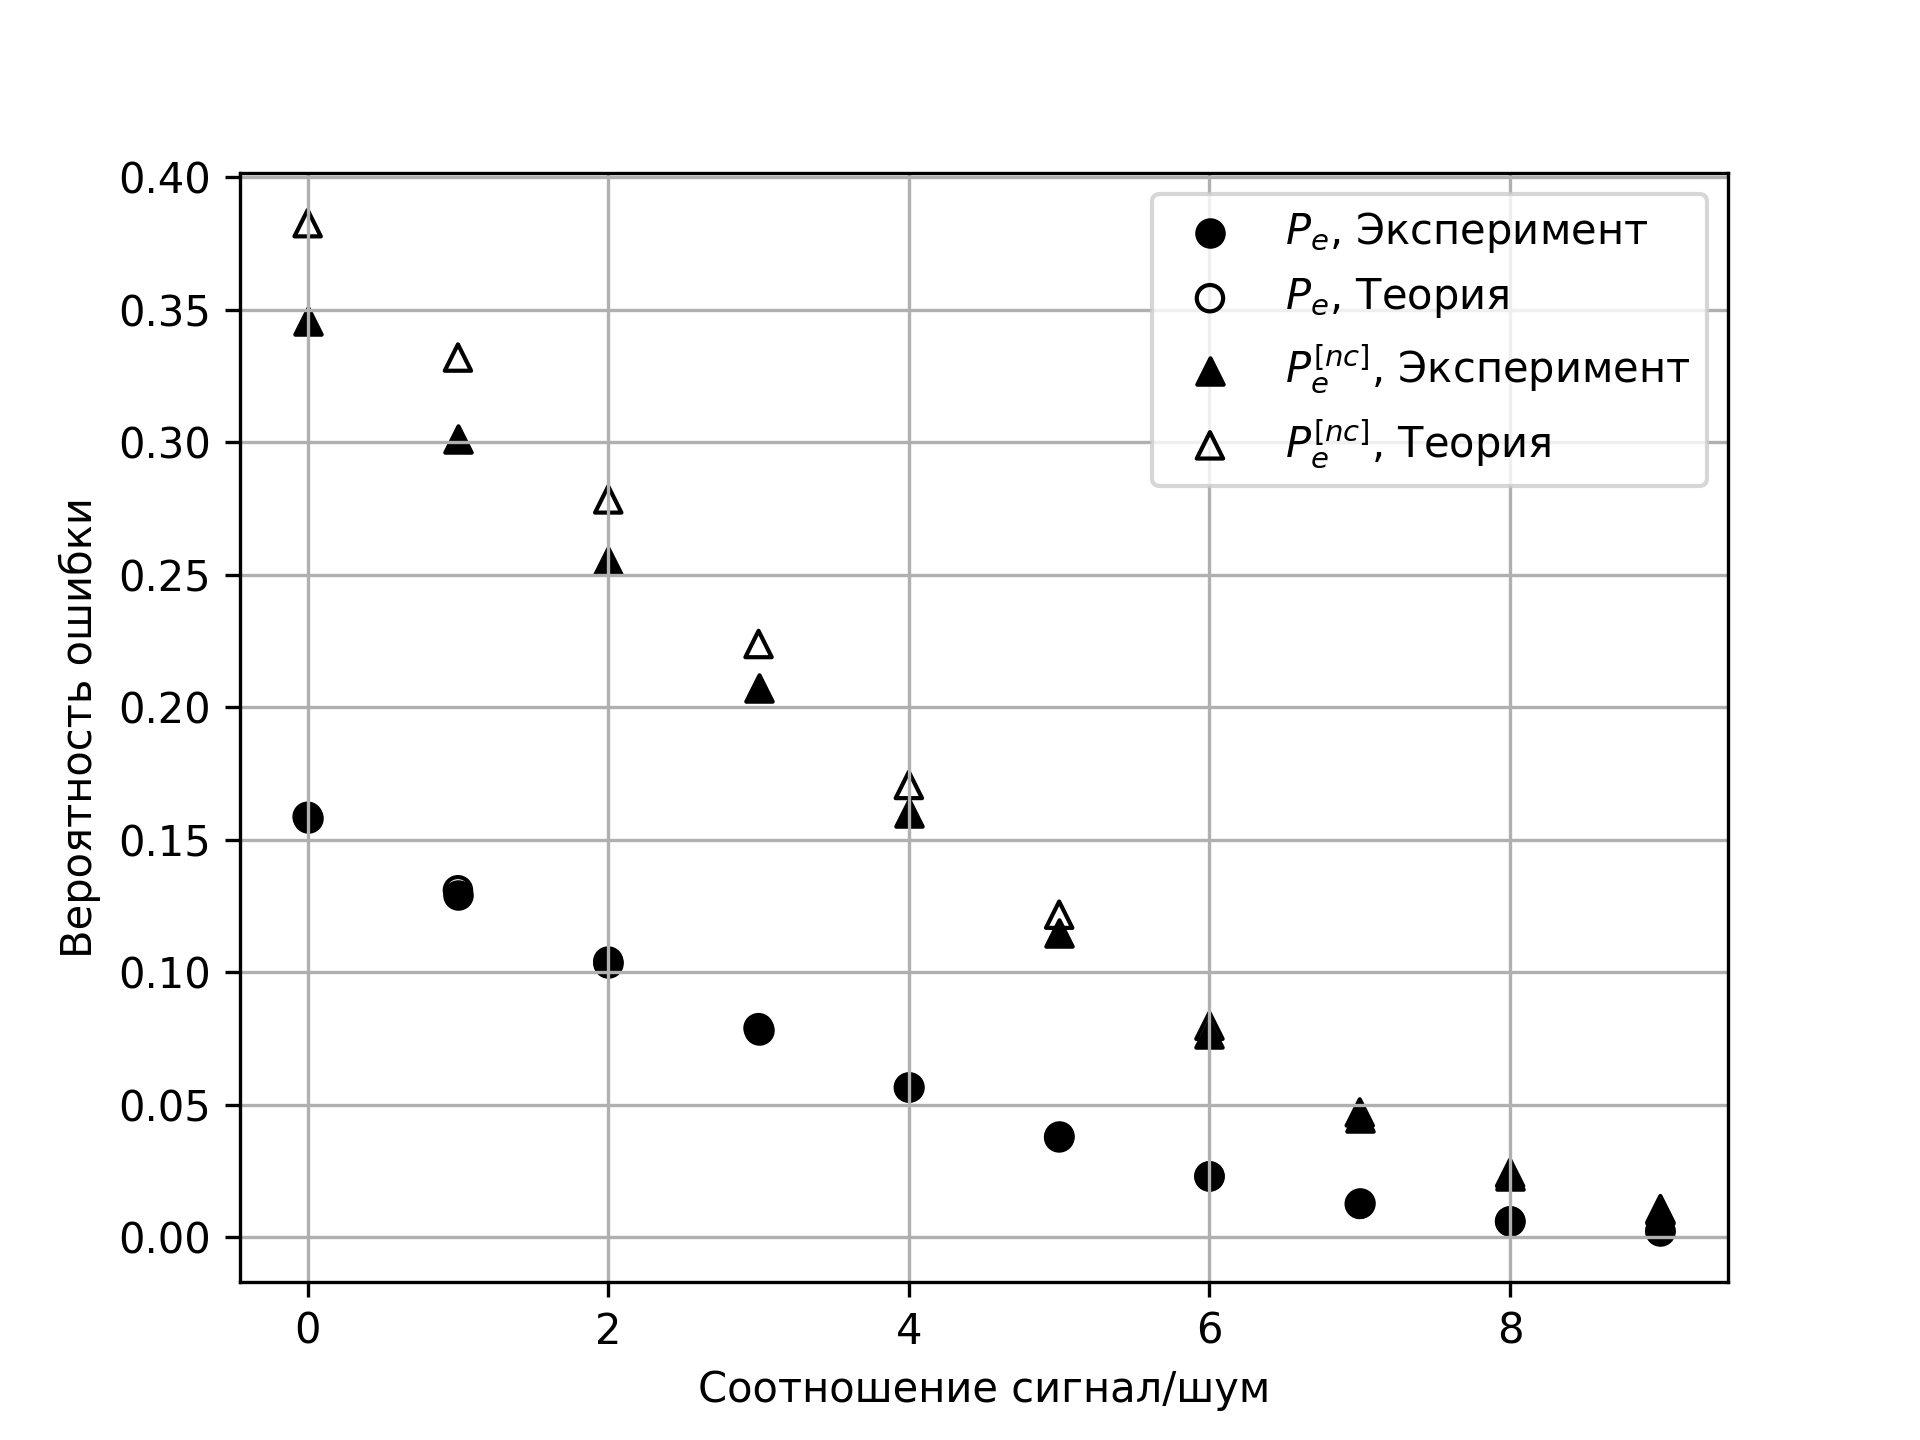
\includegraphics[width=.6\linewidth]{../images/rt2-3}
\end{figure}

\section{Канал с квадратурной модуляцией QPSK}

\begin{figure}[H]
\centering
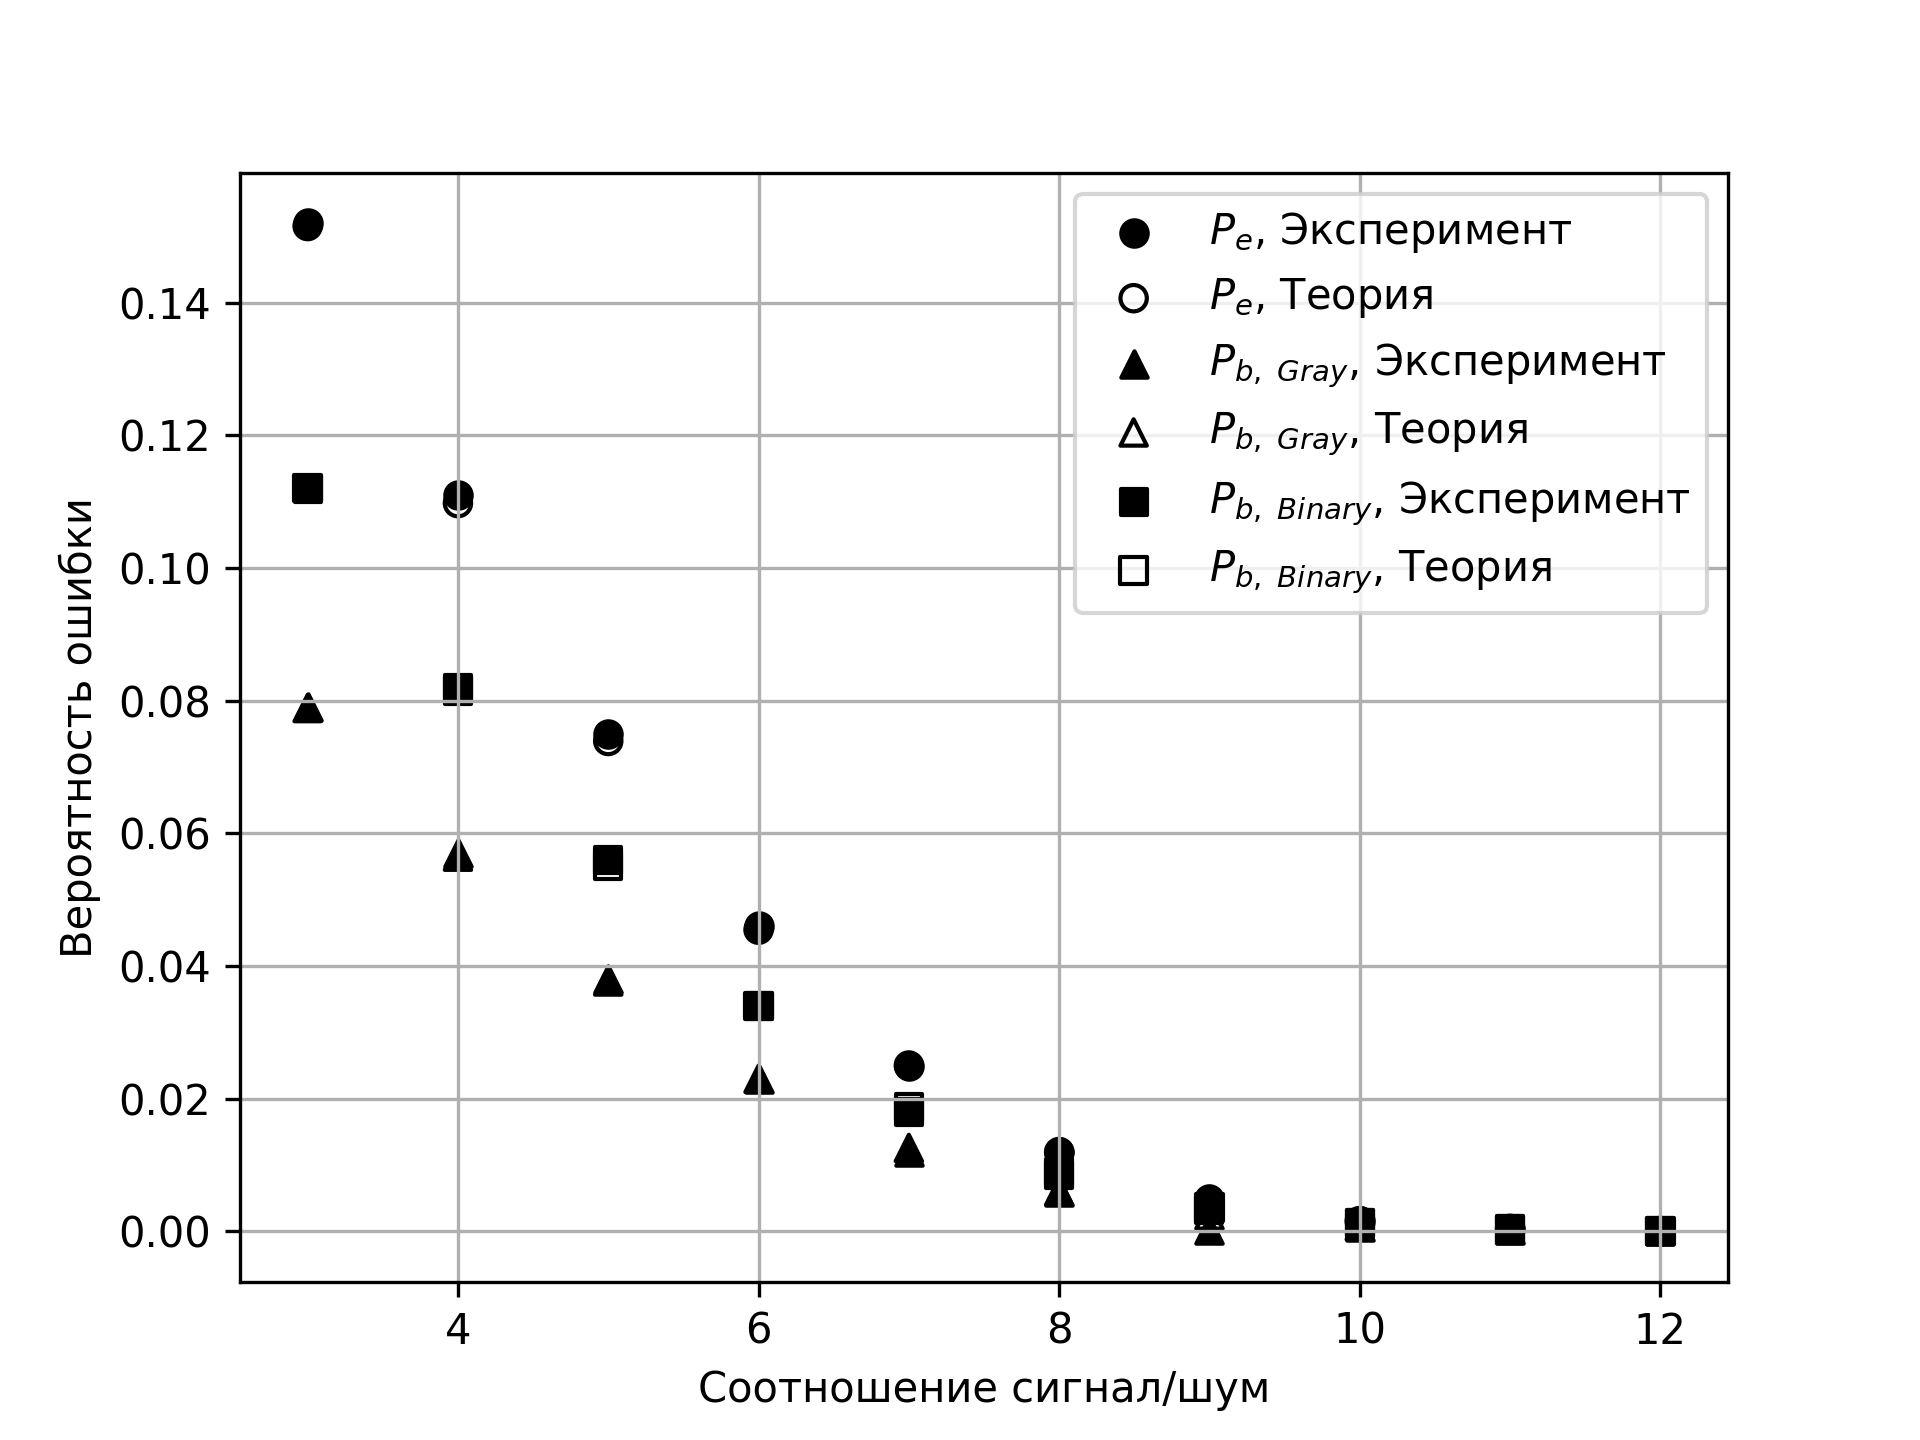
\includegraphics[width=.6\linewidth]{../images/rt2-4}
\end{figure}

Оценим выигрыш в отношении сигнал/шум, который нумерация Грея дает при $P_b\approx10^{-3}$. Для этого установим  $\text{snr}=10\ \text{dB}$. При этом вероятность ошибки на бит при Binary-нумерации составит $P_b^\prime\approx0.0012$. Затем перейдем на нумерацию Грея и будем постепенно снижать отношение сигнал/шум. При $\text{snr}=9.6\ \text{dB}$ получим ту же самую вероятность ошибки.

\section{Каналы с M-ичной модуляцией}

\begin{figure}[H]
\centering
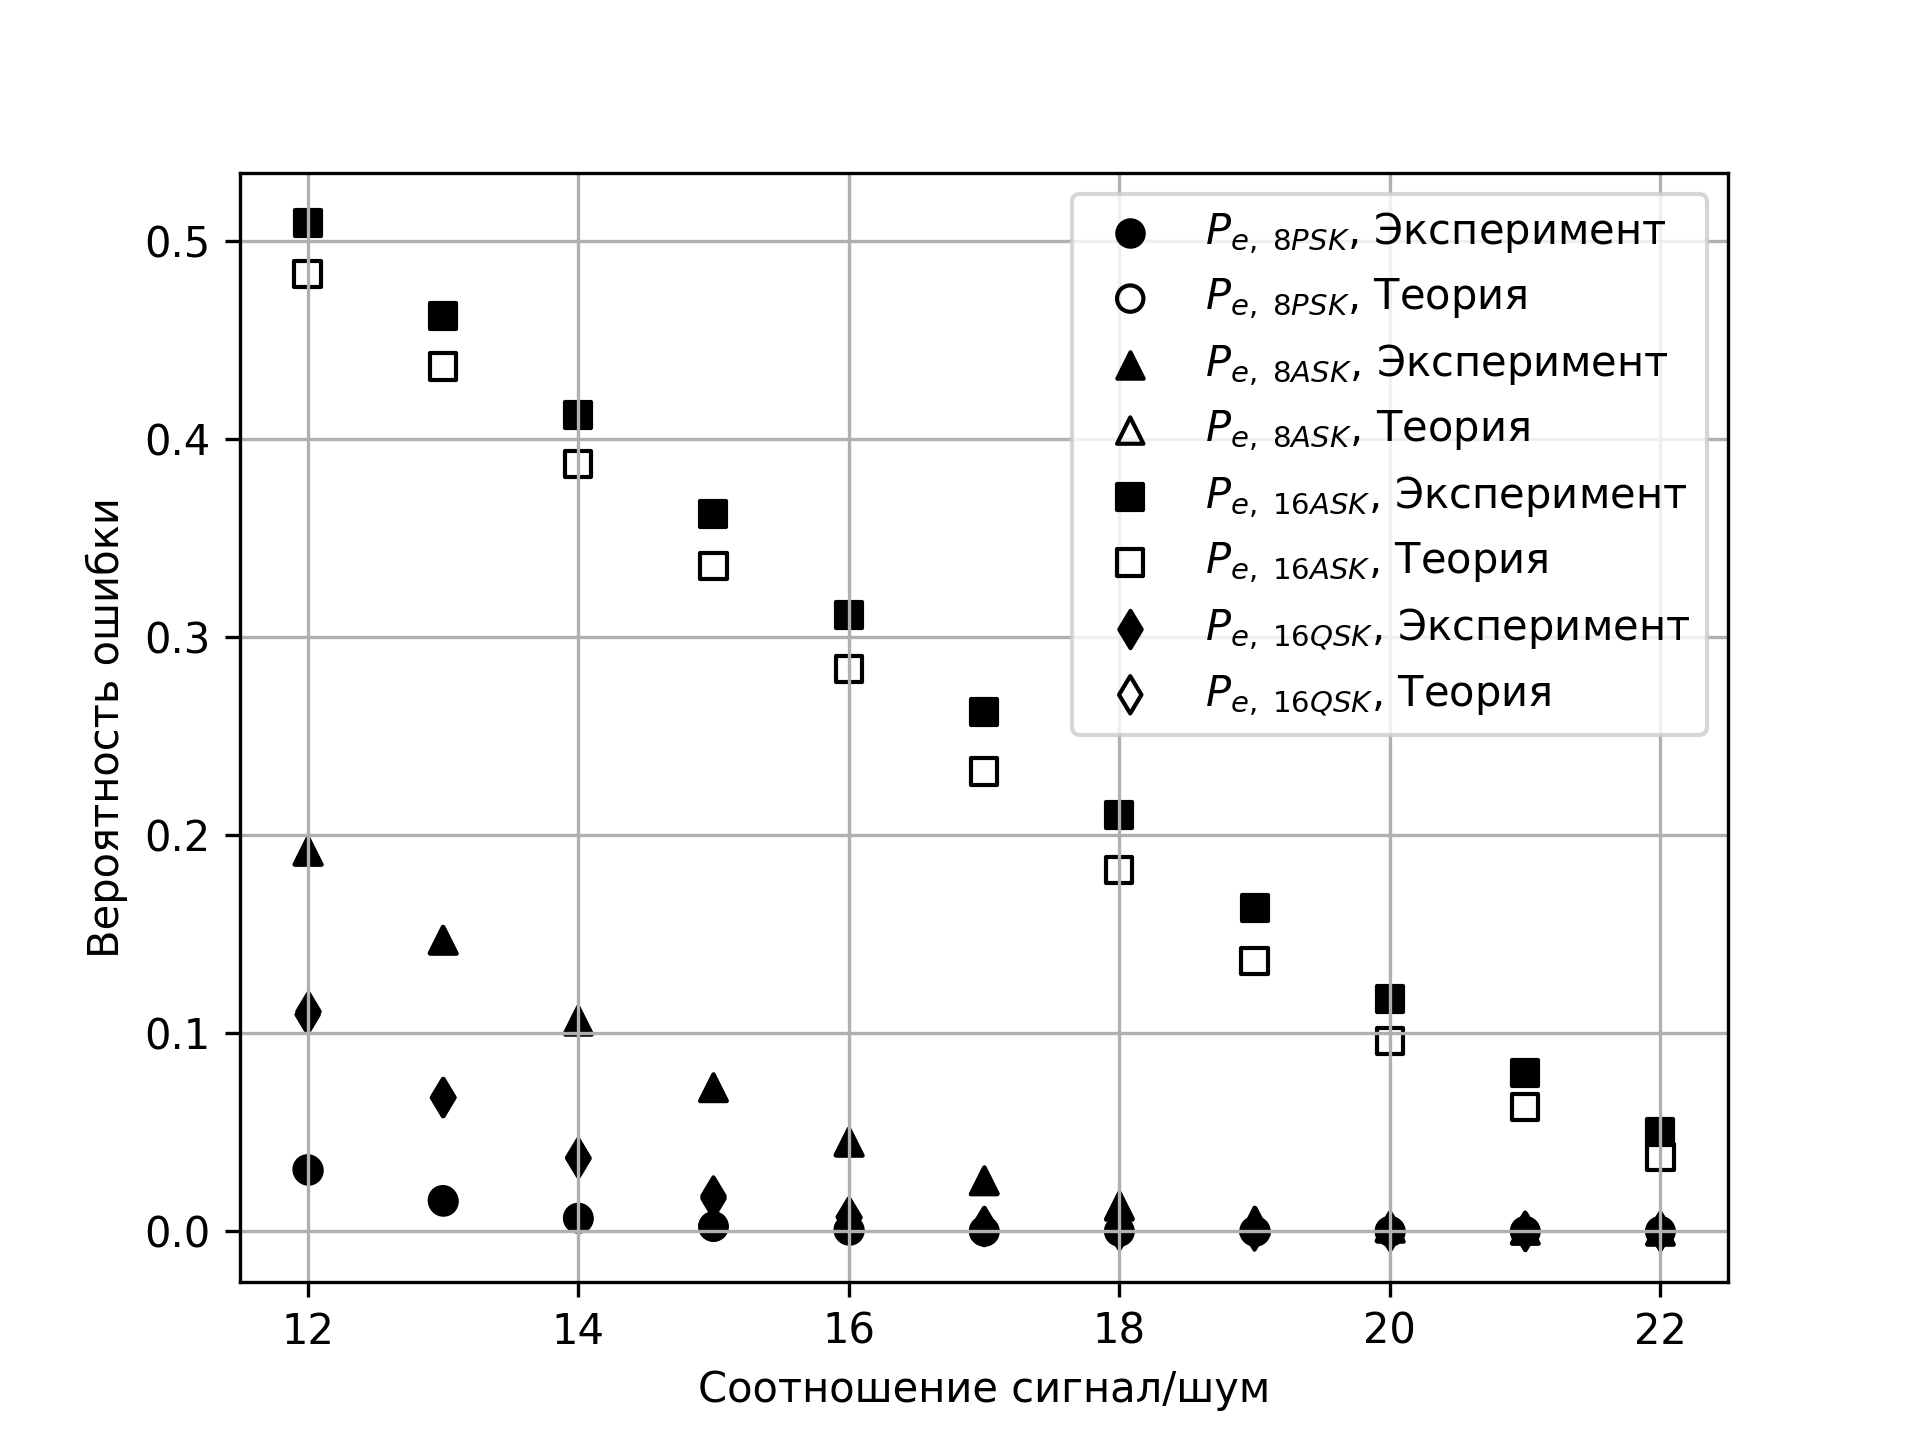
\includegraphics[width=.7\linewidth]{../images/rt2-5}
\end{figure}

Выясним насколько нужно увеличить snr, чтобы сохранить уровень $P_e\approx10^{-4}$ при переходе от 8ASK к 16ASK. Получим, что $P_{e,\ 8ASK}\approx10^{-4}$ при  $\text{snr}=22\ \text{dB}$, а $P_{e,\ 16ASK}\approx10^{-4}$ при  $\text{snr}\approx28\ \text{dB}$. Аналогично, 16ASK проигрывает 16QAM по snr примерно на $9\ \text{dB}$. А при переходе от 16QAM к 32QAM для сохранения уровня $P_e\approx10^{-4}$ необходимо увеличить snr на 3.

\section{Линейная модуляция с прямоугольным импульсом}

\begin{figure}[H]
\centering
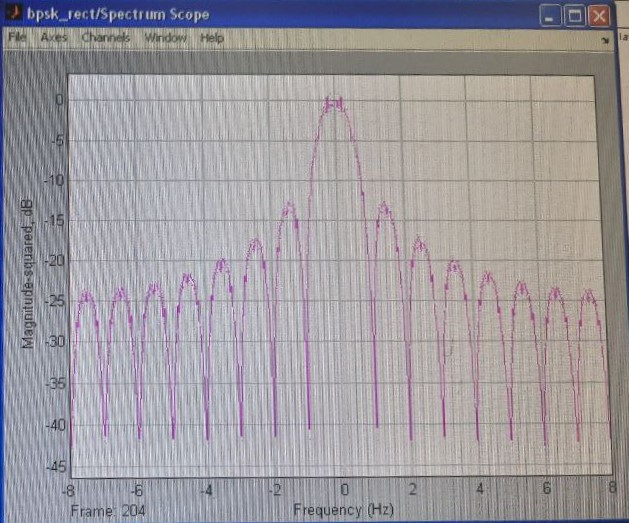
\includegraphics[width=.7\linewidth]{../images/rt2-6}
\caption{Спектр мощности сигнала ($\text{snr}=30\ \text{dB}$)}
\end{figure}

\section{Корень из приподнятого косинуса}

\begin{figure}[H]
\centering
\begin{subfigure}{.33\textwidth}
  \centering
  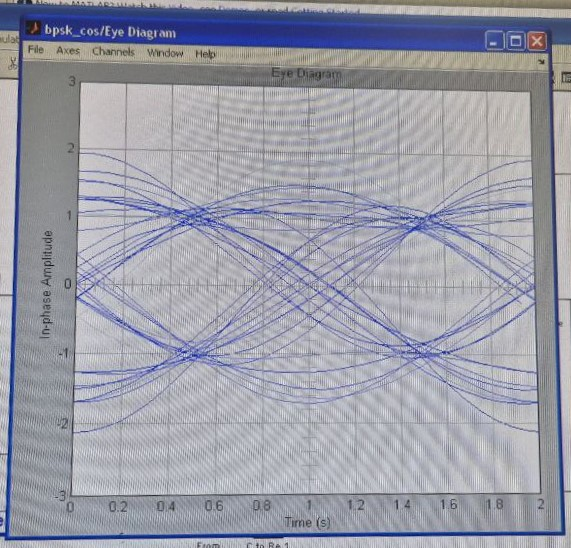
\includegraphics[width=.95\linewidth]{../images/rt2-7d}
  \caption{$m=0.1$}
\end{subfigure}%
\begin{subfigure}{.33\textwidth}
  \centering
  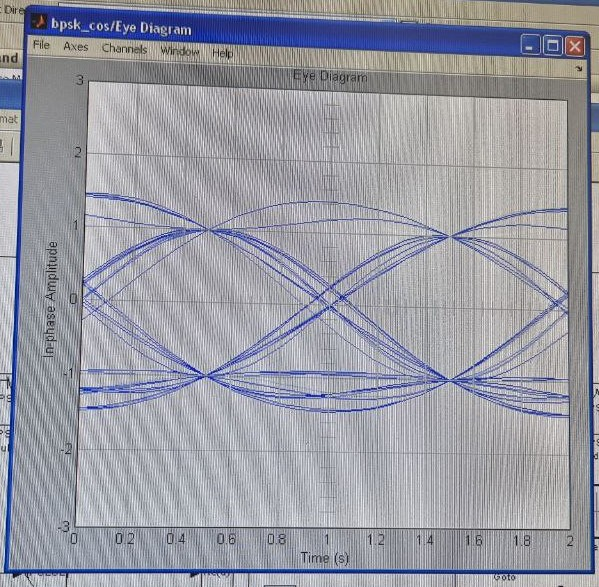
\includegraphics[width=.95\linewidth]{../images/rt2-7e}
  \caption{$m=0.5$}
\end{subfigure}
\begin{subfigure}{.33\textwidth}
  \centering
  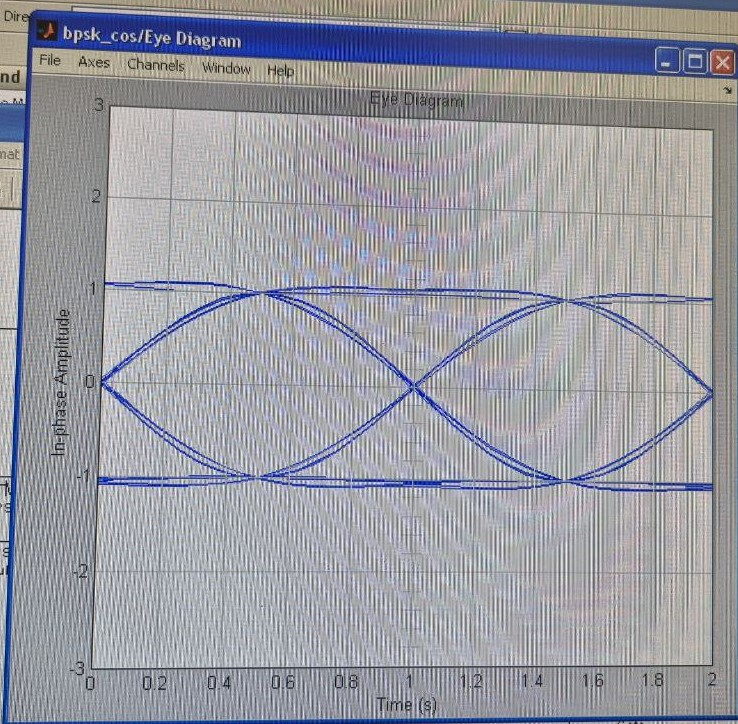
\includegraphics[width=.95\linewidth]{../images/rt2-7f}
  \caption{$m=0.9$}
\end{subfigure}%
\caption{Глазковая диаграмма при различных значениях m}
\end{figure}

\begin{figure}[H]
\centering
\begin{subfigure}{.33\textwidth}
  \centering
  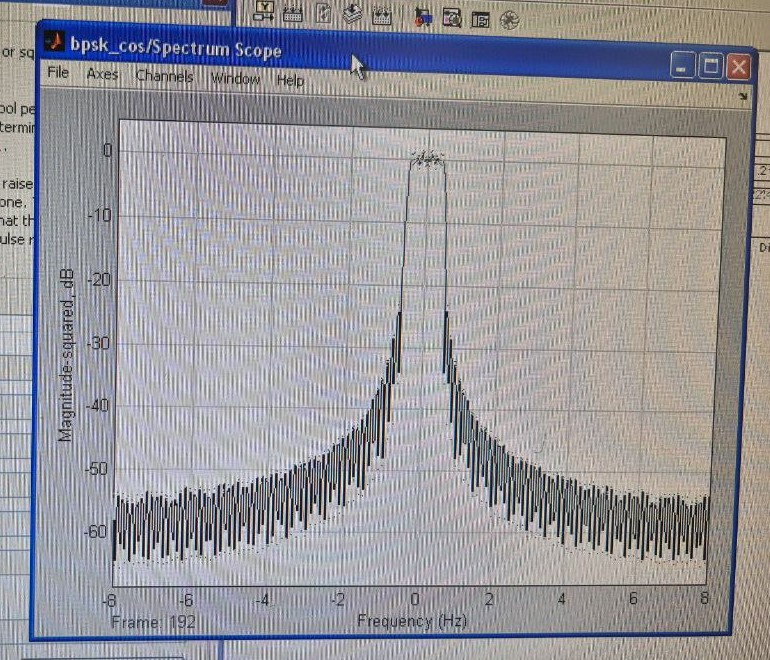
\includegraphics[width=.95\linewidth]{../images/rt2-7a}
  \caption{$m=0.1$}
\end{subfigure}%
\begin{subfigure}{.33\textwidth}
  \centering
  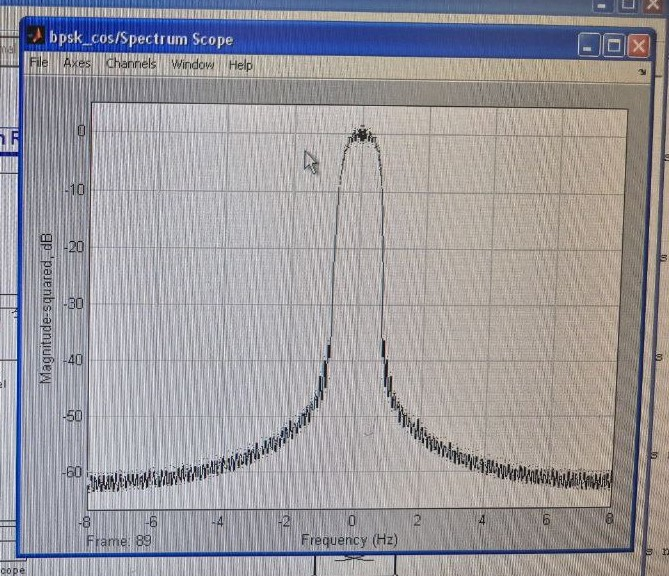
\includegraphics[width=.95\linewidth]{../images/rt2-7b}
  \caption{$m=0.5$}
\end{subfigure}
\begin{subfigure}{.33\textwidth}
  \centering
  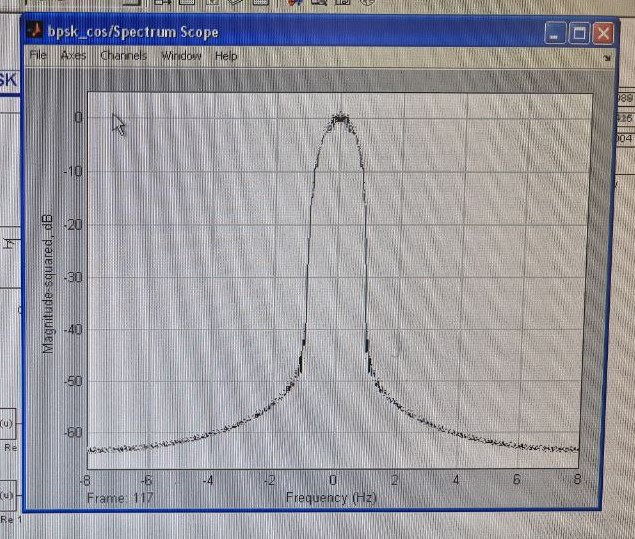
\includegraphics[width=.95\linewidth]{../images/rt2-7c}
  \caption{$m=0.9$}
\end{subfigure}%
\caption{Спектр мощности при различных значениях m}
\end{figure}

\newpage

\section{Двоичная частотная модуляция}

\begin{figure}[H]
\centering
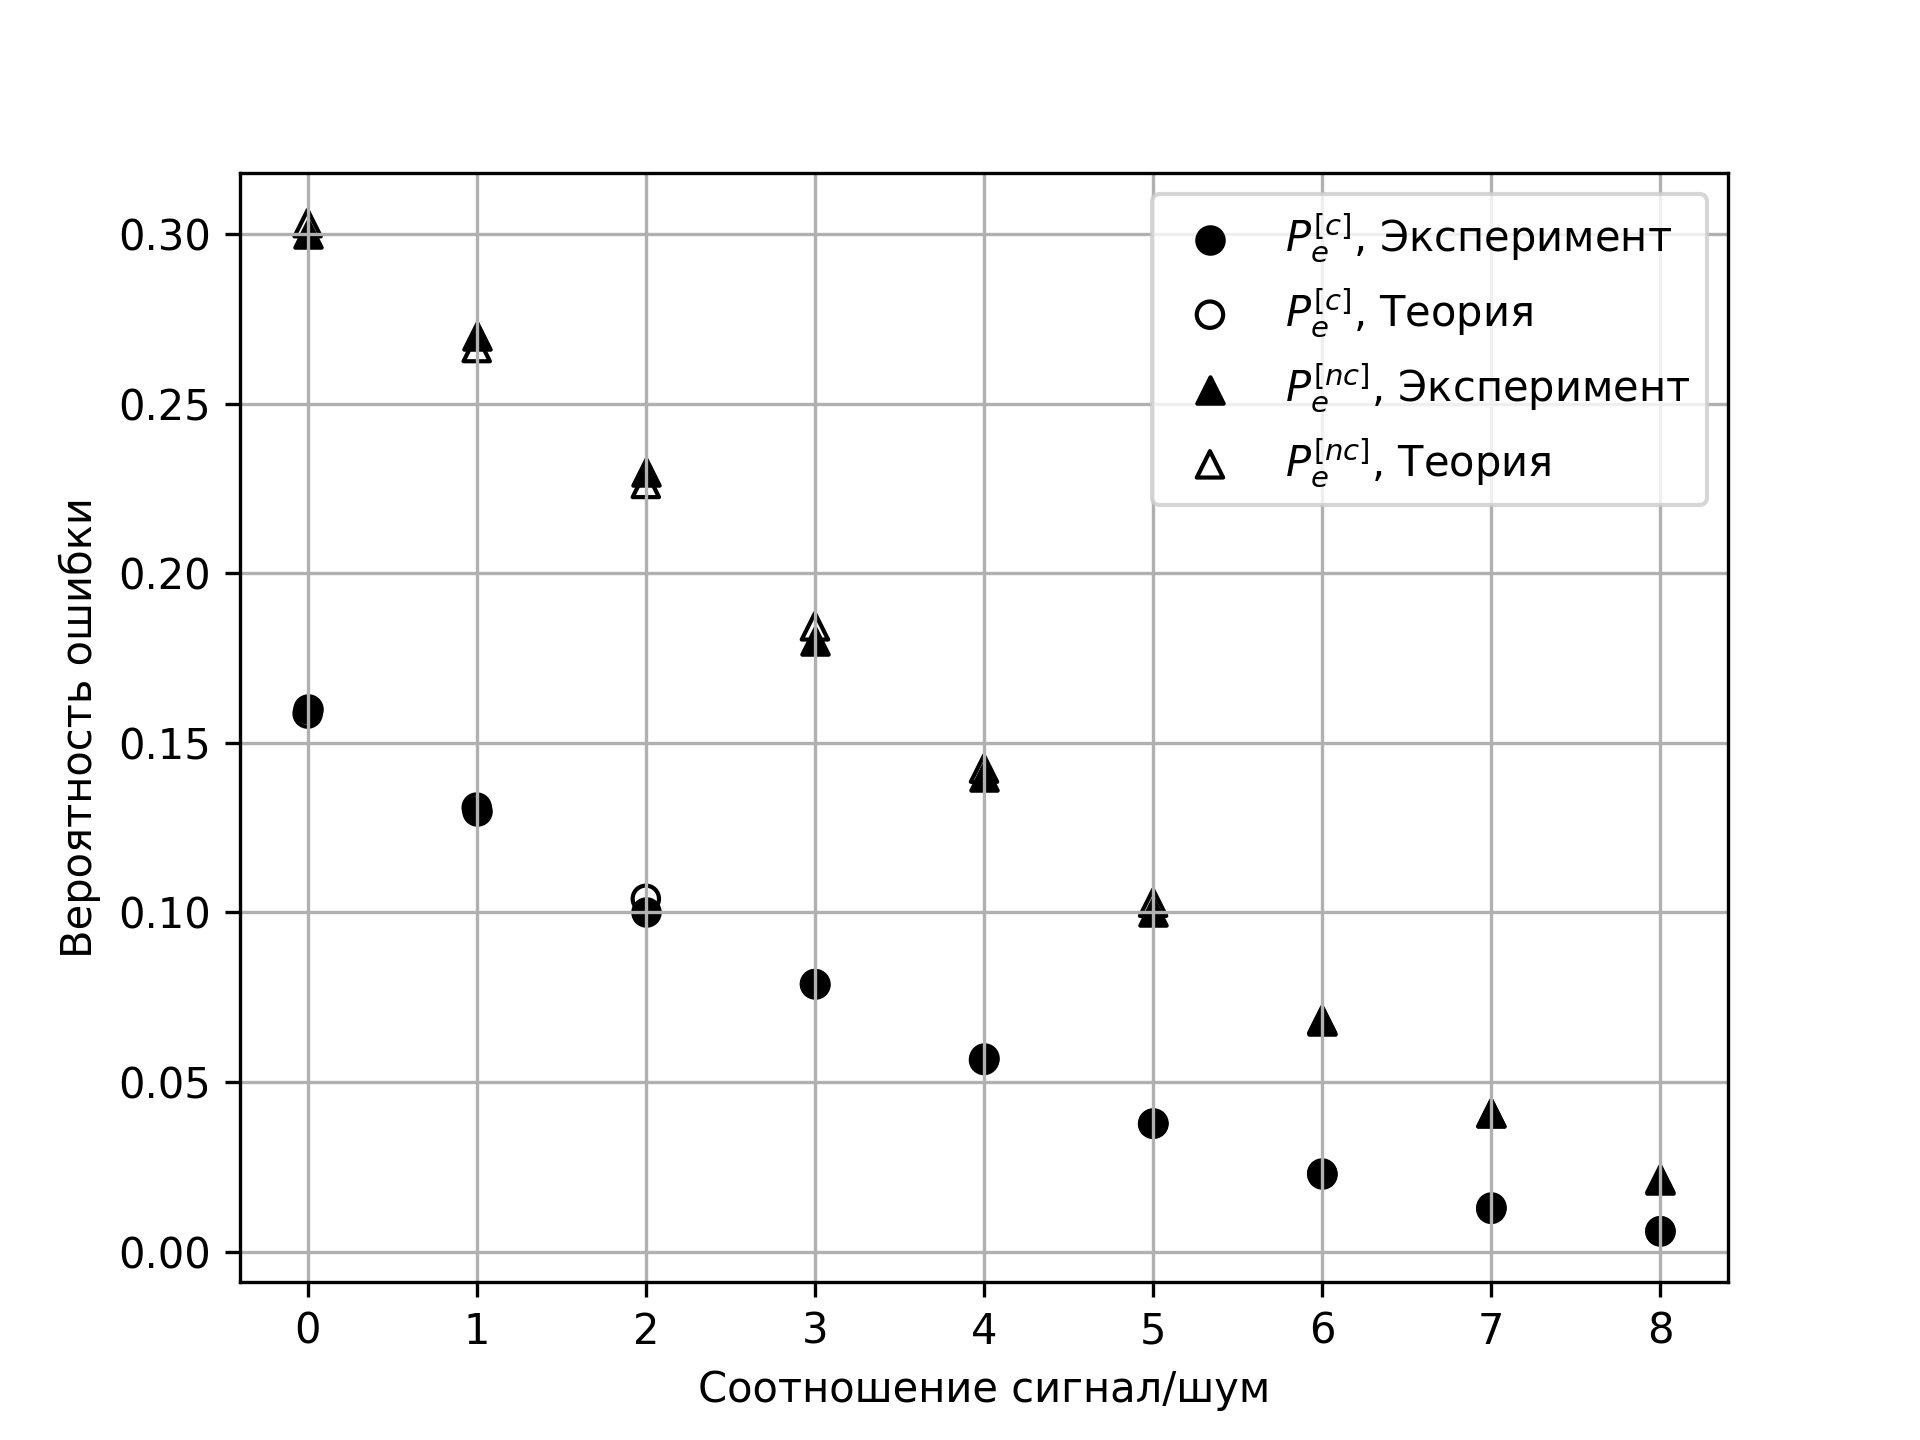
\includegraphics[width=.8\linewidth]{../images/rt2-8}
\end{figure}

\begin{figure}[H]
\centering
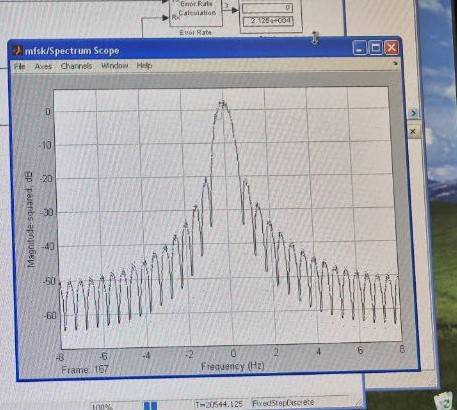
\includegraphics[width=.8\linewidth]{../images/rt2-9s}
\caption{Спектр мощности сигнала в отсутствии шума ($\text{snr}=100\ \text{dB}$)}
\end{figure}

\section{Модуляция с минимальным частотным сдвигом}

\begin{figure}[H]
\centering
\begin{subfigure}{.5\textwidth}
  \centering
  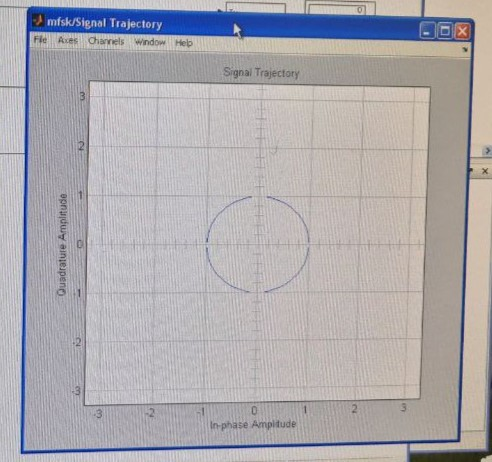
\includegraphics[width=.95\linewidth]{../images/rt2-9a}
  \caption{$\text{snr}=100\ \text{dB}$}
\end{subfigure}%
\begin{subfigure}{.5\textwidth}
  \centering
  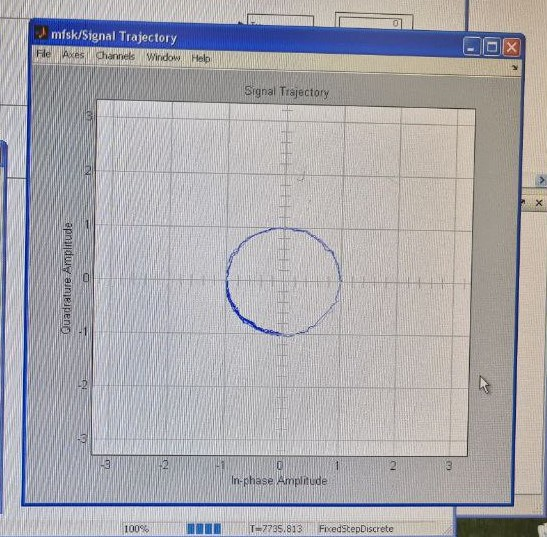
\includegraphics[width=.95\linewidth]{../images/rt2-9b}
  \caption{$\text{snr}=30\ \text{dB}$}
\end{subfigure}
\begin{subfigure}{.5\textwidth}
  \centering
  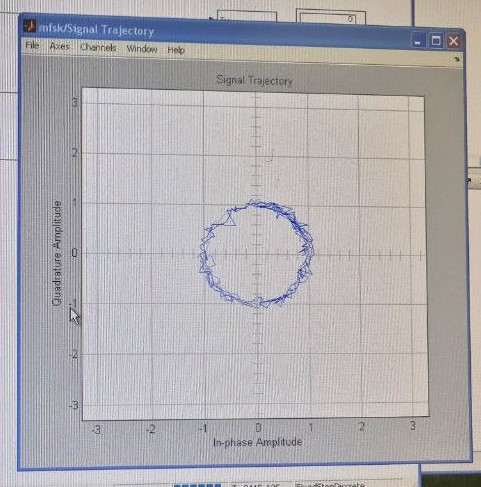
\includegraphics[width=.95\linewidth]{../images/rt2-9c}
  \caption{$\text{snr}=20\ \text{dB}$}
\end{subfigure}%
\begin{subfigure}{.5\textwidth}
  \centering
  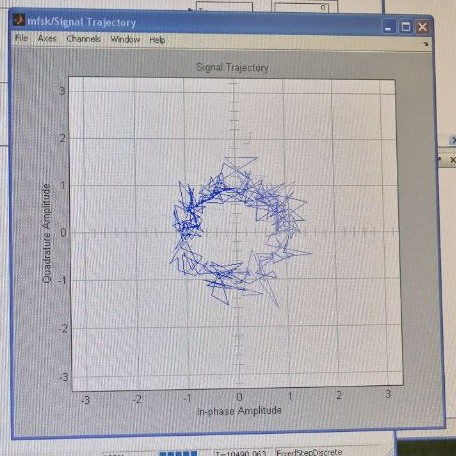
\includegraphics[width=.95\linewidth]{../images/rt2-9d}
  \caption{$\text{snr}=10\ \text{dB}$}
\end{subfigure}%
\caption{Траектория движения сигнальной точки при различных соотношениях сигнал/шум}
\end{figure}

\begin{figure}[H]
\centering
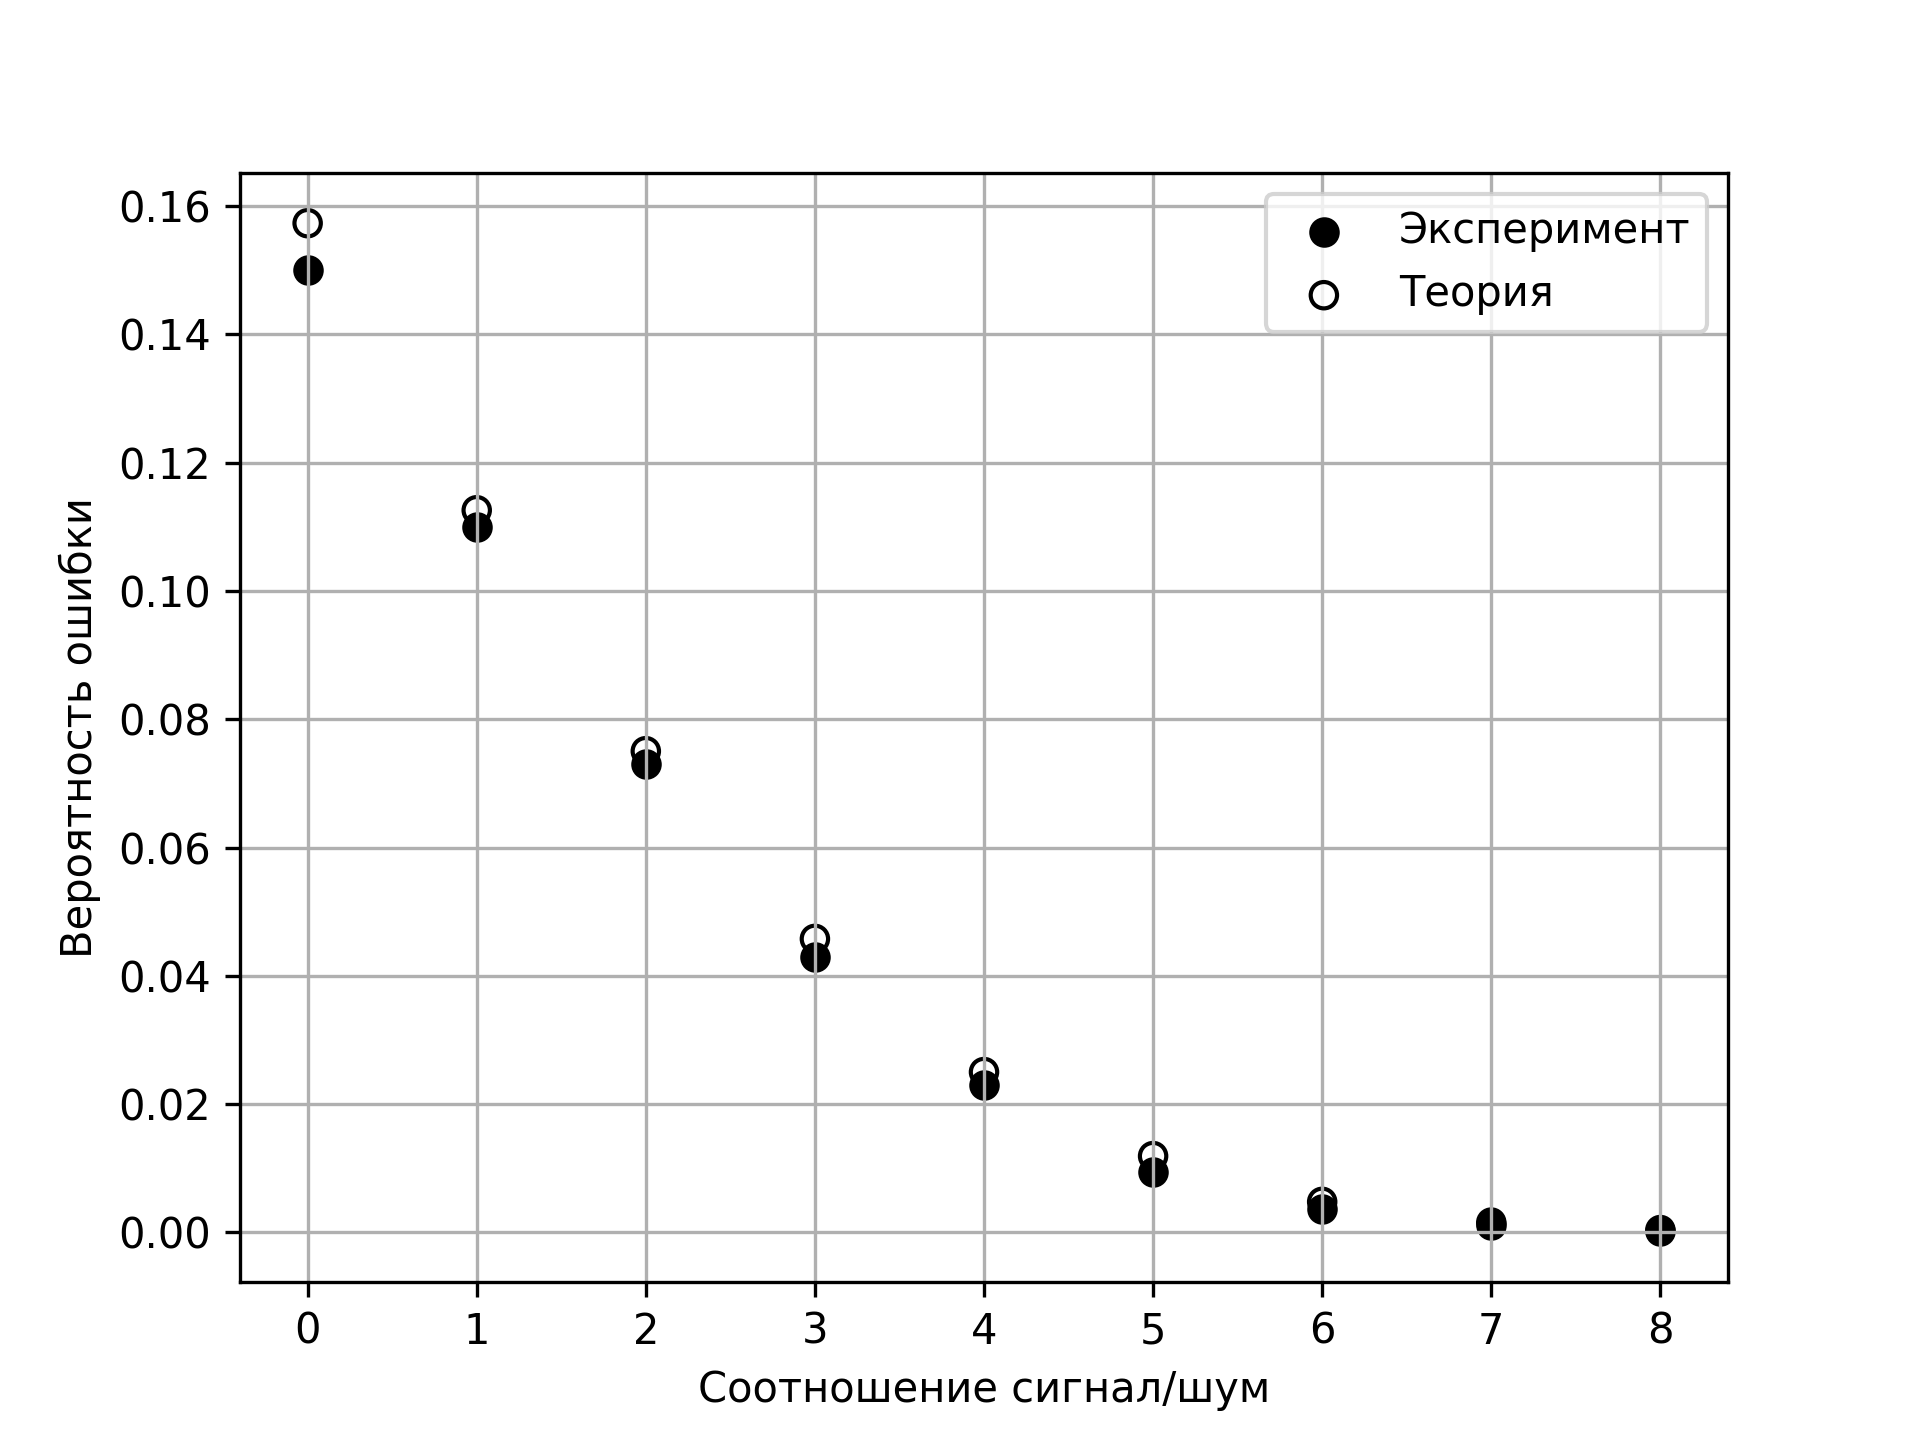
\includegraphics[width=.8\linewidth]{../images/rt2-9}
\end{figure}

\begin{figure}[H]
\centering
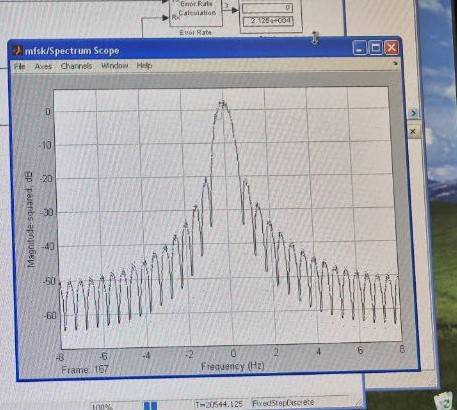
\includegraphics[width=.8\linewidth]{../images/rt2-9s}
\caption{Спектр мощности сигнала в отсутствии шума ($\text{snr}=100\ \text{dB}$)}
\end{figure}

\end{document}